\documentclass{article}
\usepackage{graphicx}
\usepackage[export]{adjustbox}
\usepackage[a4paper, left = 1cm, right = 1cm, top = 3cm, bottom = 1.25cm]{geometry}

%% Path to images
\graphicspath{ {./images/} }

\begin{document}

\title{\vspace{-4cm}Experimental Design for the Testing of a New Golf Ball}
\author{Trent Henderson}
\date{}

\maketitle

As a company who is increasingly focused on amateur golfers, Titleist are interested in understanding the performance of their new ball relative to their existing ball, especially for high handicap players\footnote{The golf handicap system in Australia ranges from 0 to 36, with tiers for "low handicap" including 0-10, "mid handicap" including 11-20, and "high handicap" including 21 and above.}. 
As such, the following research question was developed: \textit{Does Titleist's new ball design improve spin rates around the green for players who currently play the standard Titleist ball?} 
Since low handicap players are highly skilled, we hypothesise that the new design would make a more marked improvement in spin rates for high and mid handicap players who are more reliant on technology to aid performance.

\subsection*{Participants}

A minimum of fifty golfers who are players of the current Titleist ball. 
Participants will be recruited via marketing emails from the official Titleist account, meaning they will comprise a relative convenience sample. 
Demographic data collected about the participants will include their handicap (numeric and grouping), age (integer measured in years), sex (categorical factor with three levels: Male, Female, Other/Intersex), and stiffness of golf club shaft (categorical factor with four levels: Seniors, Regular, Stiff, Extra Stiff). 
Participants will be required to have hit no other balls on the testing day.

\subsection*{Materials}

\begin{itemize}
    \item 25x current golf ball (5 for warm-up) per player
    \item 25x new golf ball (5 for warm-up) per player
    \item 1x 60 degree lob wedge per player
    \item GC Quad ball tracker with TrackMan software per player
\end{itemize}

\subsection*{Procedure}

Each participant will randomly hit ten balls from a single bucket, where five are the current Titleist ball and five are the new ball. 
Following the warm-up, each participant will then randomly hit forty balls from a single bucket, where twenty are the current Titleist ball and twenty are the new ball.
All balls for both warm-up and testing will be mixed in the same bucket and unmarked to avoid any participant equipment bias, but will be electronically marked so that the computer software will be able to detect ball type. 
The response variable \textit{spin rate} will be measured via a launch monitor which can accurately track spin (and other statistics) for each shot. 
Testing will occur over the course of one week and even numbers of players from all three handicap groupings will be recruited for each day to counterbalance any methodological effects.

\subsection*{Statistical Analysis}

It is proposed that a generalised linear model with a gamma or lognormal link function (due to spin values only being positive) will be fit to the data, with ball type, handicap grouping, a set of control variables (age, sex, shaft stiffness), and an interaction term between ball type and handicap grouping will be included as predictors. 
Hypothetically, if the research question is supported, results similar to the simulation presented in Figure~\ref{fig:expectations} would be expected.
Evidently, the relative gain in spin rate for the new ball (after controlling for other variables) is much lower for high handicappers, but is quite substantial for mid and especially low handicappers. 
More simply, the new ball's technology may help high handicappers to experience performance closer to those with higher skill.

\begin{figure}[h]
    \centering
    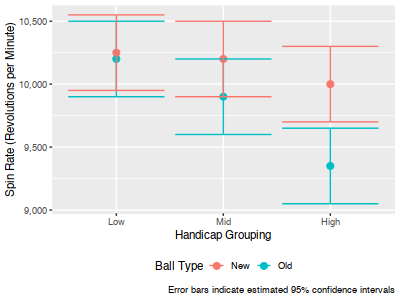
\includegraphics[max width=\linewidth, scale=0.53]{expectations}
    \caption{\label{fig:expectations}Hypothesised relationship between ball type and handicap grouping}
\end{figure}

\end{document}